\chapter{Условие}%
\label{cha:uslovie}

\section{Задание 1}
\label{sec:task_1}

Назначить адреса подсетей:

\begin{enumerate}
    \item Подсеть 1: 192.168.12.0 /24
    \item Подсеть 2: 192.168.13.0 /24
    \item Подсеть 3: 192.168.14.0 /24
\end{enumerate}

\section{Задание 2}
\label{sec:task_2}

Настроить поддержку трех виртуальных локальных сетей (VLan 10, 20, 30) на коммутаторе.

\section{Задание 3}
\label{sec:task_3}

Настроить маршрутизацию между виртуальными локальными сетями на маршрутизаторе.

\section{Задание 4}
\label{sec:task_4}

Выделить и озаглавить на схеме каждую виртуальную локальную сеть.

\chapter{Практическая часть}%
\label{cha:prakticheskaia_chast_}

\section{Задача 1}%
\label{sec:1}

В рамках первого задания были назначены адреса подсетей в соответствии с условием.

\section{Задача 2}%
\label{sec:2}

Во время выполнения второго задания была настроена поддержка трёх виртуальных сетей на коммутаторе. На рисунках ниже представлены команды, которые выполнялись на коммутаторе.

\begin{figure}[H]
    \centering
    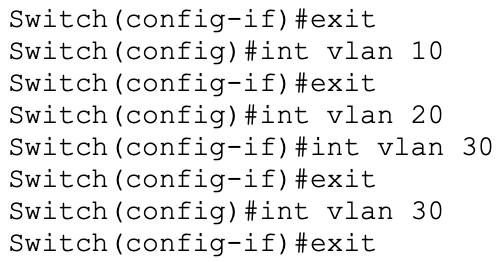
\includegraphics[width=0.7\textwidth]{images/img-1.png}
    \caption{Настройка коммутатора. Часть 1}
    \label{fig:router7}
\end{figure}

\begin{figure}[H]
    \centering
    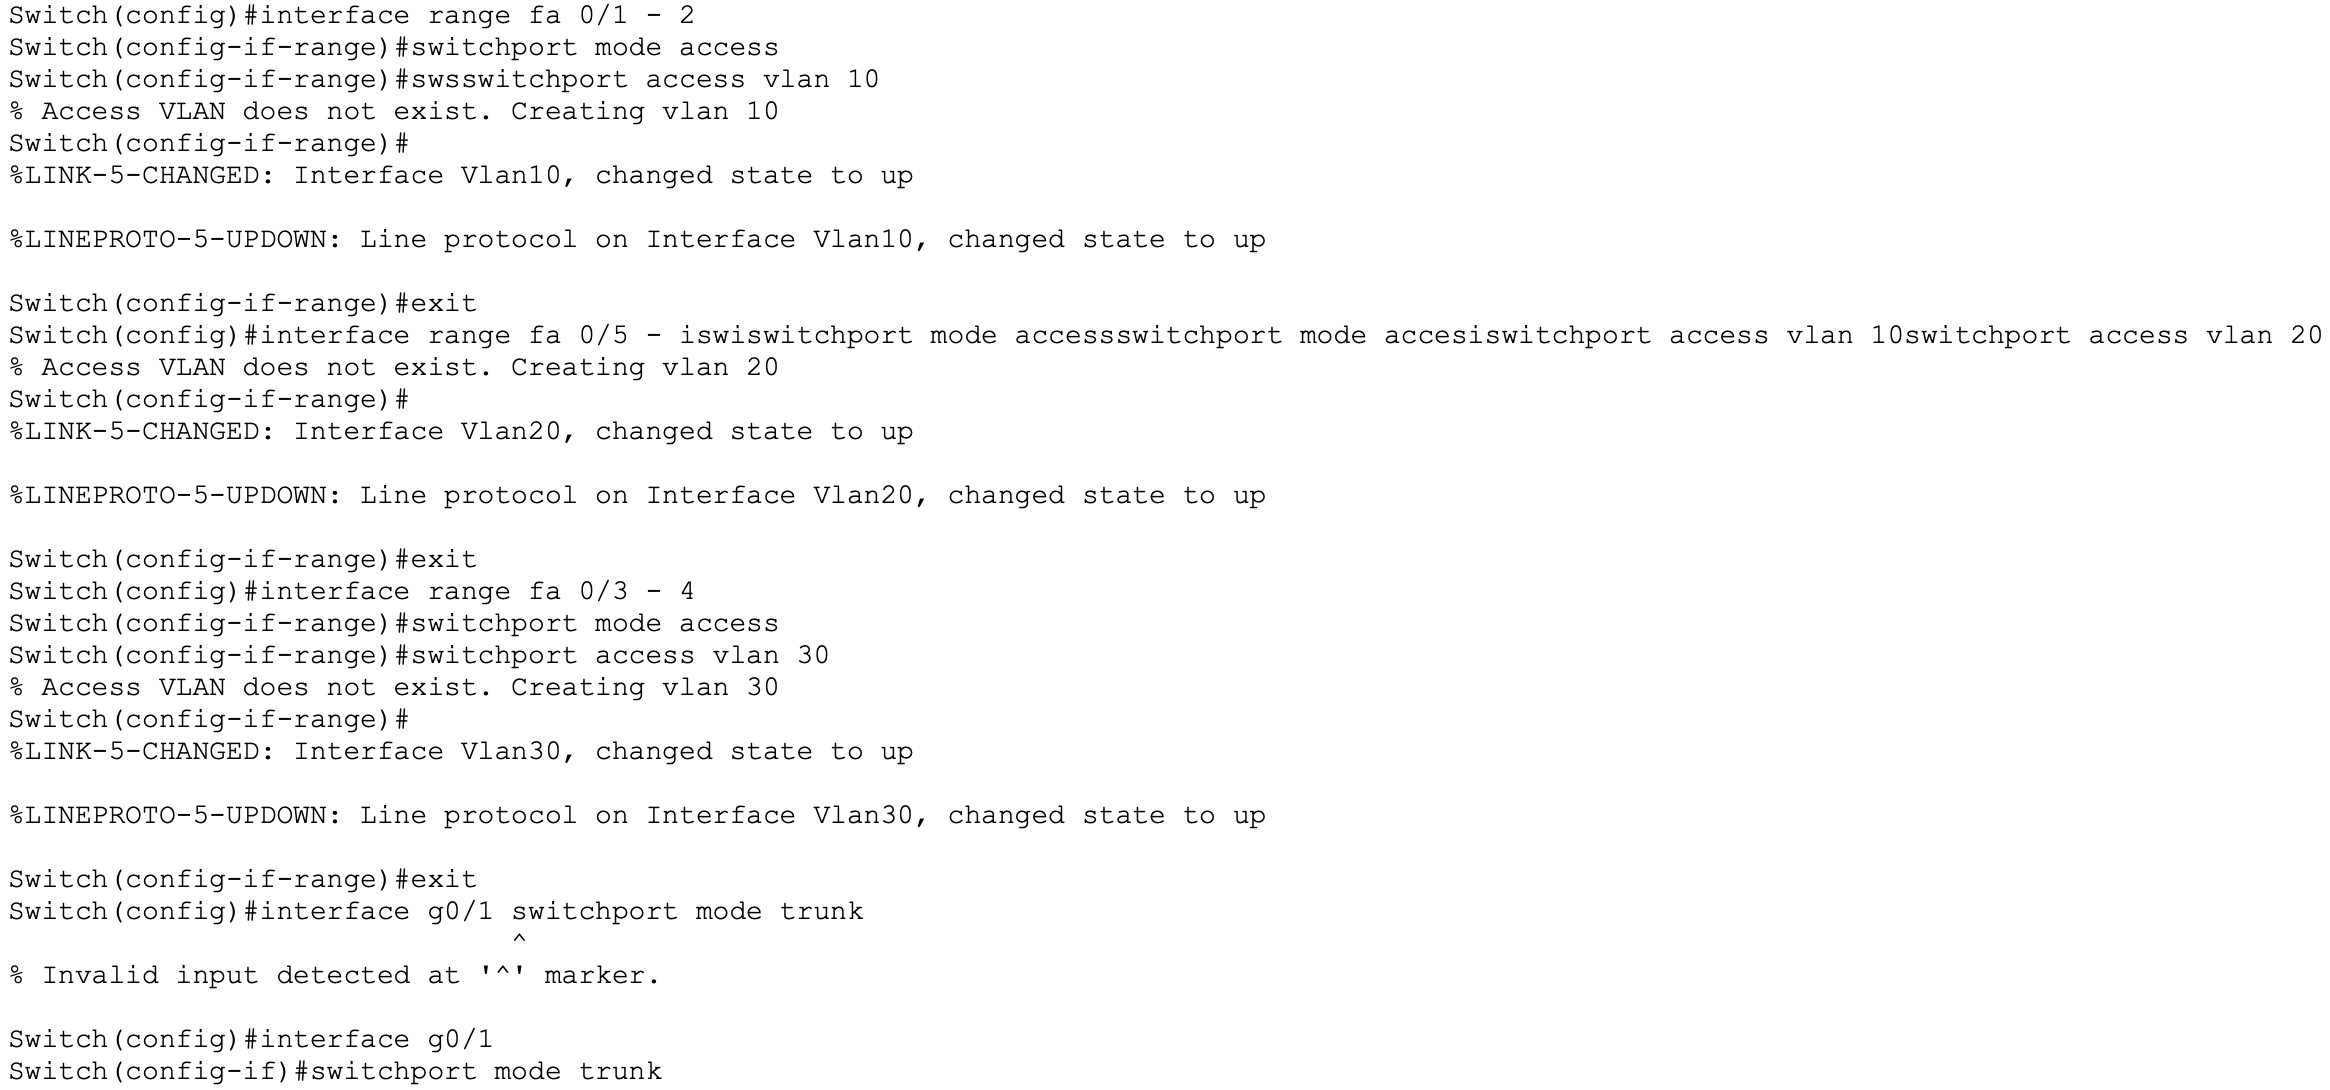
\includegraphics[width=1.04\textwidth]{images/img-2.png}
    \caption{Настройка коммутатора. Часть 2}
    \label{fig:router7}
\end{figure}

После выполнения вышеприведенных команд были добавлены vlan10, vlan20 и vlan30, что видно на рисунке ниже.

\begin{figure}[H]
    \centering
    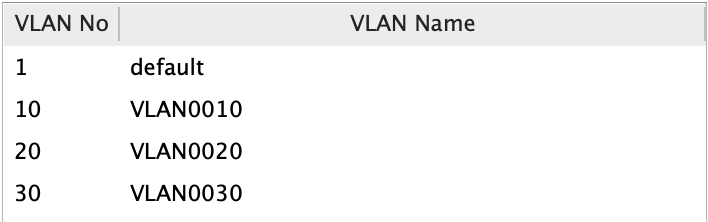
\includegraphics[width=1\textwidth]{images/vlan.png}
    \caption{Список виртуальных сетей на коммутаторе}
    \label{fig:router7}
\end{figure}

На рисунке ниже видно, что также в результате выполнения этих команд для физических интерфейсов было указано, для какой виртуальной сети передавать данные.

\begin{figure}[H]
    \centering
    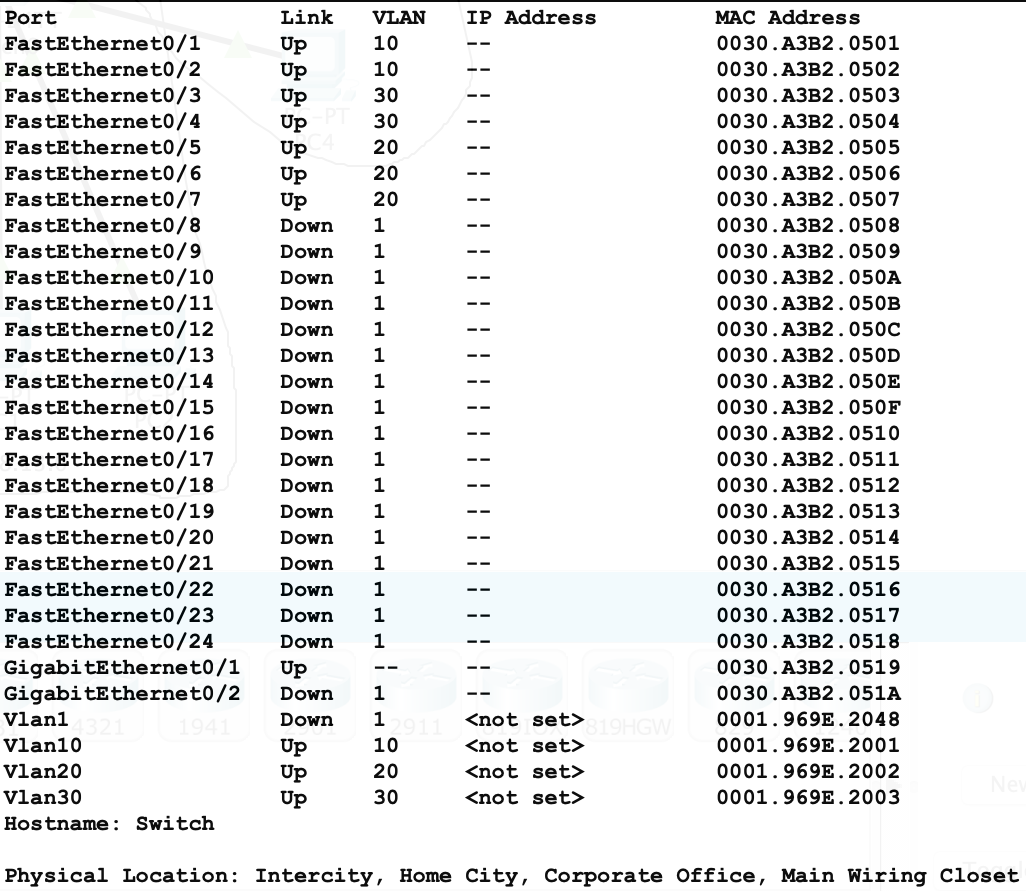
\includegraphics[width=1\textwidth]{images/switch-int.png}
    \caption{Список физических интерфейсов коммутатора}
    \label{fig:router7}
\end{figure}

\section{Задача 3}%
\label{sec:3}

Во время настройки маршрутизации между виртуальными локальными сетями на маршрутизаторе выполнялись команды, представленные на рисунках ниже.

\begin{figure}[H]
    \centering
    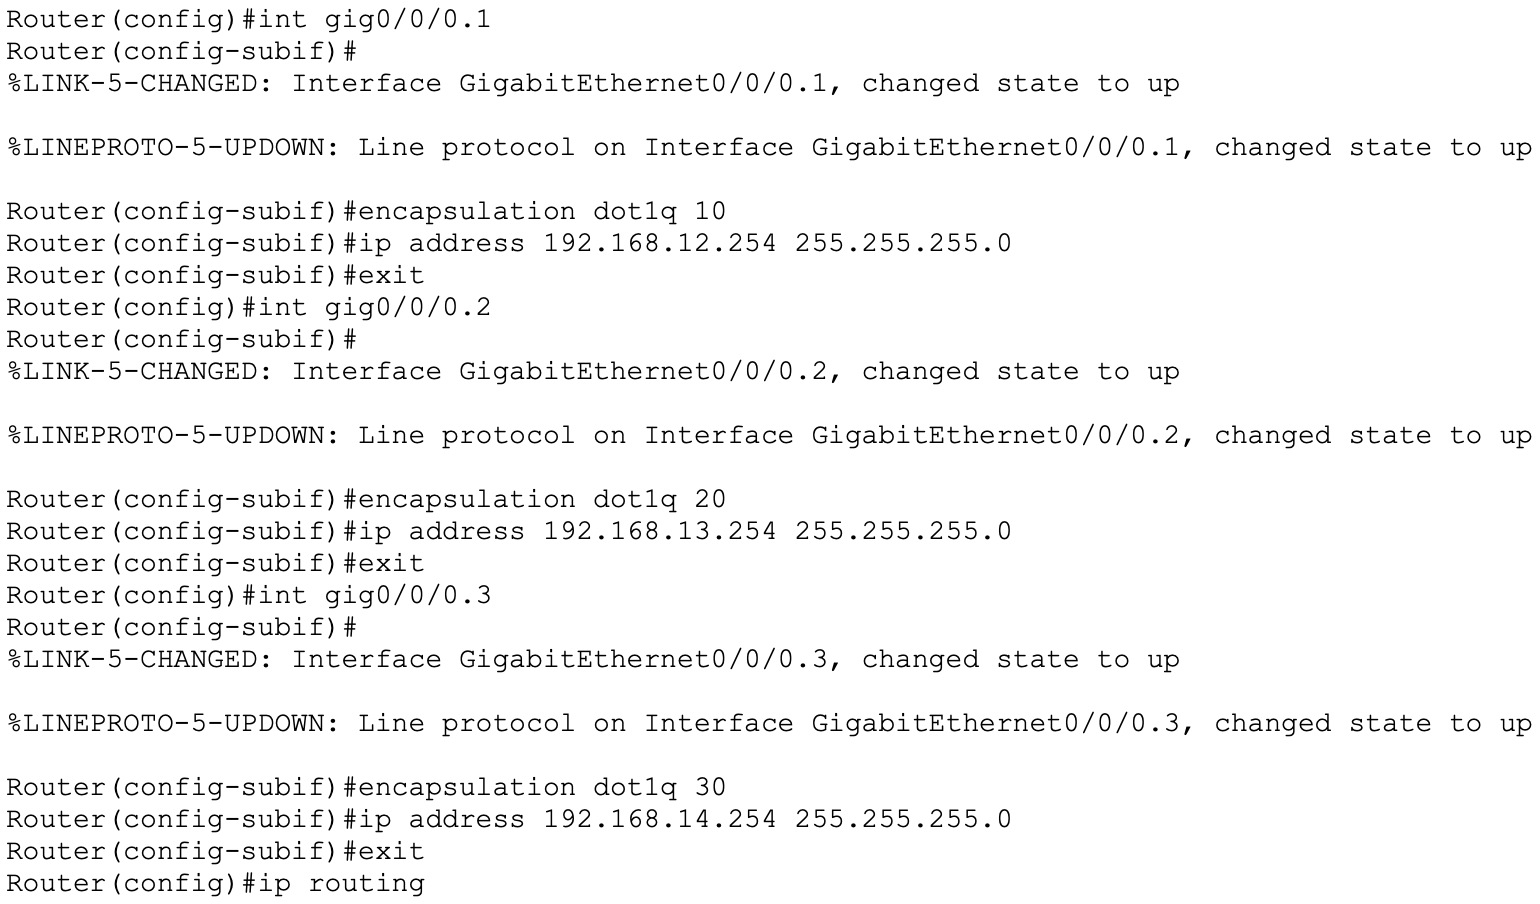
\includegraphics[width=1\textwidth]{images/task-3.png}
    \caption{Команды для настройки маршрутизатора}
    \label{fig:router7}
\end{figure}

После выполнения этих команд были созданы три подинтерфейса, что показано на рисунке ниже.

\begin{figure}[H]
    \centering
    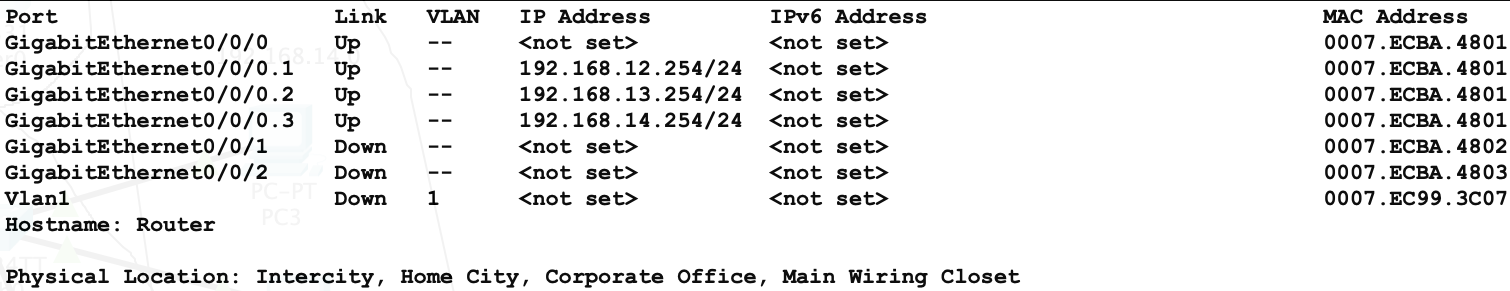
\includegraphics[width=1\textwidth]{images/task-3-2.png}
    \caption{Список интерфейсов маршрутизатора}
    \label{fig:router7}
\end{figure}

\section{Задача 4}%
\label{sec:4}

На рисунке ниже изображены выделенные виртуальные сети.

\begin{figure}[H]
    \centering
    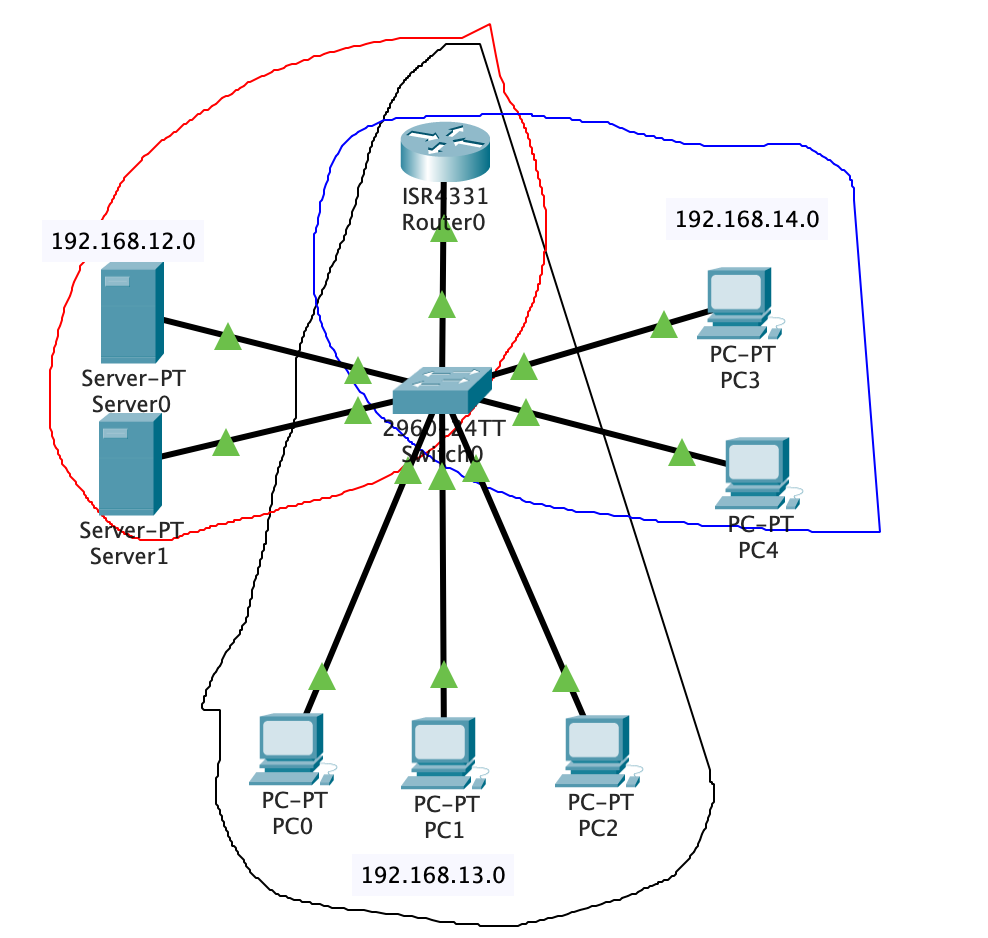
\includegraphics[width=1\textwidth]{images/shema.png}
    \caption{Выделенные виртуальные сети}
    \label{fig:router7}
\end{figure}

На рисунке ниже представлен результат команды ping, сделанной из PC4 в Server1.
\begin{figure}[H]
    \centering
    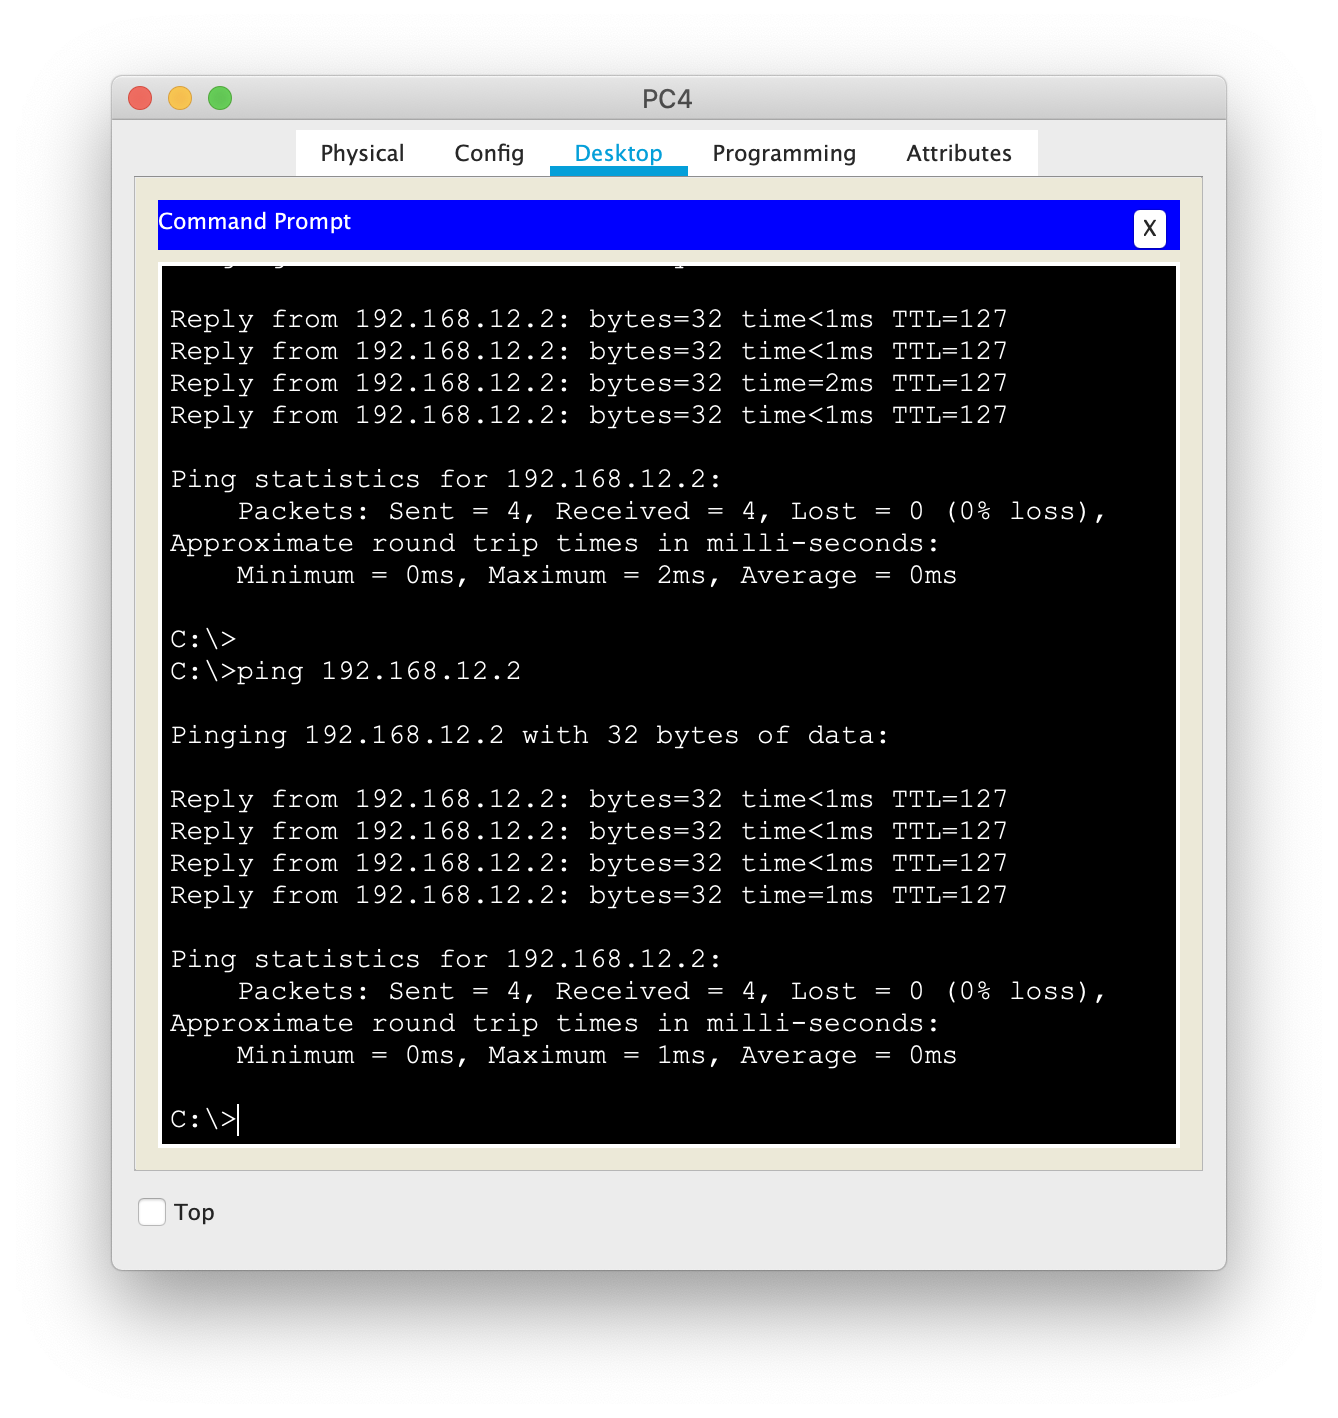
\includegraphics[width=1\textwidth]{images/ping.png}
    \caption{Результат проверки соединения}
    \label{fig:router7}
\end{figure}
